\documentclass[12pt]{article}
\usepackage[margin=1in]{geometry}
\usepackage[all]{xy}


\usepackage{amsmath,amsthm,amssymb,color,latexsym}
\usepackage{geometry}        
\geometry{letterpaper}    
\usepackage{graphicx}

\usepackage{listings}
\usepackage[english]{babel}
\usepackage[export]{adjustbox}
\usepackage[table,xcdraw]{xcolor}

\definecolor{codegreen}{rgb}{0,0.6,0}
\definecolor{codegray}{rgb}{0.5,0.5,0.5}
\definecolor{codepurple}{rgb}{0.58,0,0.82}
\definecolor{backcolour}{rgb}{0.95,0.95,0.92}

\lstdefinestyle{mystyle}{
  backgroundcolor=\color{backcolour},   commentstyle=\color{codegreen},
  keywordstyle=\color{magenta},
  numberstyle=\tiny\color{codegray},
  stringstyle=\color{codepurple},
  basicstyle=\ttfamily\footnotesize,
  breakatwhitespace=false,         
  breaklines=true,                 
  captionpos=b,                    
  keepspaces=true,                 
  numbers=left,                    
  numbersep=5pt,                  
  showspaces=false,                
  showstringspaces=false,
  showtabs=false,                  
  tabsize=2
}

\lstset{style=mystyle}

\usepackage{graphicx}
\graphicspath{ {./images/} }


\newtheorem{problem}{Problem}

\newenvironment{solution}[1][\it{Solution}]{\textbf{#1. } }{$\square$}


\begin{document}
\noindent CS 6140: Machine Learning Spring 2021\hfill Committee Machines\\
Sai Nikhil (04/29/2021)\hfill thirandas.s@northeastern.edu

\hrulefill


\begin{problem}
This exercise will help you give a good understanding of the differences between bagging and boosting, with implementation.

a) What are the major differences between boosting and bagging?\\

b) Prove the following upper bound result for training error of AdaBoost.\\

Assume $\epsilon_{t}<\frac{1}{2}$ and let $\gamma_{t}=\frac{1}{2}-\epsilon_{t} .$ Then the following bound holds
$$
\frac{1}{n}\left|\left\{i: f\left(x_{i}\right) \neq y_{i}\right\}\right| \leq \prod_{t=1}^{T} \sqrt{1-4 \gamma_{t}^{2}} \leq e^{-2 \sum_{t=1}^{T} \gamma_{t}^{2}}
$$
where, $\epsilon_{t}$ is the training error of expert $f_t(x)$.\\

c) Implement a Random Forest and Boosting Classifier for a classification dataset from UCI Machine Learning Repository. Discuss the whole experimentation process.
\end{problem}
\begin{solution}

a)


\begin{table}[h]
\centering
\begin{tabular}{|l|l|}
\hline
\rowcolor[HTML]{EFEFEF} 
Bagging                                                                                                                                        & Boosting                                                                                                                                                                                                      \\ \hline
\begin{tabular}[c]{@{}l@{}}The ensembled model is built from\\  individual experts independently.\end{tabular}                                 & \begin{tabular}[c]{@{}l@{}}The ensembled model is built by\\  adding new models that do well\\  where the previous models fail.\end{tabular}                                                                  \\ \hline
This can happen parallelly.                                                                                                                    & This has to happen sequentially.                                                                                                                                                                              \\ \hline
\begin{tabular}[c]{@{}l@{}}The final output is an equal weighted\\  average/majority vote of the output\\  of individual experts.\end{tabular} & \begin{tabular}[c]{@{}l@{}}The final output is weighted average\\  with a learnt probability distribution\\  where more weight is given to those\\  with better performance on training\\  data.\end{tabular} \\ \hline
Tries to reduce over-fitting problem.                                                                                                          & Reduces bias.                                                                                                                                                                                                 \\ \hline
\end{tabular}
\end{table}


b) 

The algorithm we saw for AdaBoost in class, is as follows:

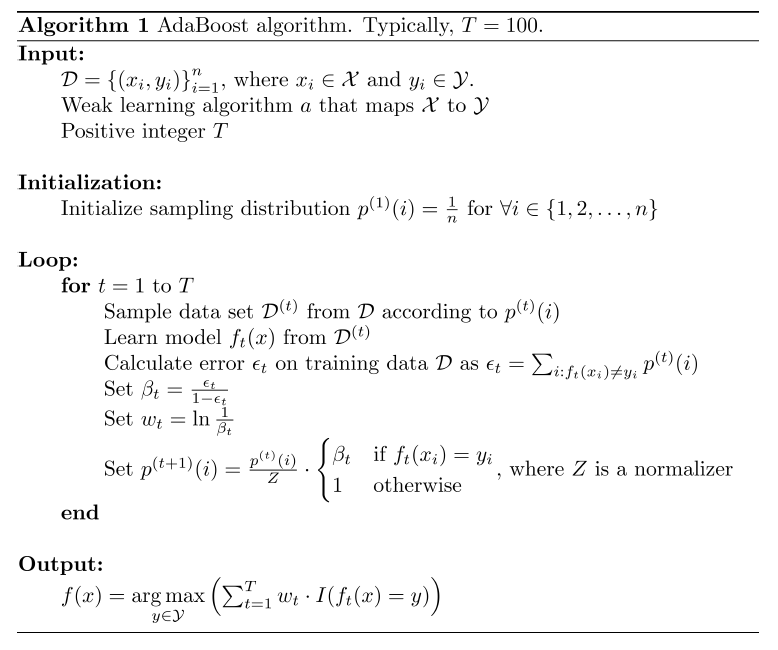
\includegraphics[scale=0.6]{AdaBoost}


For a classification scenario,

Output of final classifier is, $f(x)=\underset{y \in \mathcal{Y}}{\arg \max }\left(\sum_{t=1}^{T} w_{t} \cdot I\left(f_{t}(x)=y\right)\right)$.


Let $y \in \{0, 1\}$. We have,\\

$
p^{(t+1)}(i)=\frac{p^{(t)}(i)}{Z_t} \cdot\left\{\begin{array}{ll}\beta_{t} & \text { if } f_{t}\left(x_{i}\right)=y_{i} \\ 1 & \text { otherwise }\end{array}\right.
$, where $Z_t$ is a normalizer
\\

This can be written as,

$$p^{(t+1)}(i)=\frac{p^{(t)}(i)e^{-w_ty_if_t\left(x_i\right)}}{Z_t}$$

Unwrapping the recursion, we get,

\begin{align*}
p^{(T)}(i) &= p^{(1)}(i) \cdot \frac{e^{-w_1y_if_1\left(x_i\right)}}{Z_1} \ldots \frac{e^{-w_{T-1}y_if_{T-1}\left(x_i\right)}}{Z_{T-1}}\\
			 &= \frac{1}{N} \cdot \frac{e^{-y_i \sum_t{w_tf_t\left(x_i\right)}}}{\prod_{t} Z_t}\\
			 &= \frac{1}{N} \cdot \frac{e^{-y_if(x_i) }}{\prod_{t} Z_t}
\end{align*}

Let us consider training error.

$$
\text { training error }(f)=\frac{1}{N} \sum_{i}\left\{\begin{array}{ll}
1 & \text { if } y_{i} \neq f\left(x_{i}\right) \\
0 & \text { else }
\end{array}\right.\\
$$
$$
=\frac{1}{N} \sum_{i}\left\{\begin{array}{ll}
1 & \text { if } y_{i} f\left(x_{i}\right) \leq 0 \\
0 & \text { else }
\end{array}\right.
$$
$$
\leq \frac{1}{N} \sum_{i} \exp \left(-y_{i} f\left(x_{i}\right)\right) \quad \text { since } e^{-z} \geq 1 \text { if } z \leq 0
$$
$$
\begin{array}{l}
=\sum_{i} p^{(T)}(i) \prod_{t} Z_{t} \\\\
=\prod_{t} Z_{t}
\end{array}
$$

The normalization constant can be computed as follows:

$$
Z_{t}=\sum_{i} p^{(t)}(i) \times\left\{\begin{array}{ll}
e^{-w_{t}} & \text { if } f_{t}\left(x_{i}\right)=y_{i} \\
1 & \text { if } f_{t}\left(x_{i}\right) \neq y_{i}
\end{array}\right.
$$
$$
=\sum_{i: f_{t}\left(x_{i}\right)=y_{i}} p^{(t)}(i) e^{-w_{t}} + \sum_{i: f_{t}\left(x_{i}\right)\ne y_{i}} p^{(t)}(i)
$$
$$
=e^{-w_{t}}(1-\epsilon_t)+\epsilon_t
$$
$$
=2\epsilon_t
$$
$$
=1-\gamma_t
$$
$$
\le e^{-\gamma_t}
$$

where, the last inequality comes from $1 + x \le e^{x}$ for all real $x$.


Substituting this in training error, we get,

$$
\frac{1}{n}\left|\left\{i: f\left(x_{i}\right) \neq y_{i}\right\}\right| = \prod_{t=1}^{T} (1-\gamma_{t}) \leq e^{-\sum_{t=1}^{T} \gamma_{t}}
$$

where, $\epsilon_{t}$ is the training error of expert $f_t(x)$.\\\\

If we choose, $y \in \{-1, +1\}$ and slightly change the algorithm like below, we get the desired result as stated in the class. 
\begin{enumerate}
\item We need to take $w_t = \frac{1}{2}\ln(\frac{1}{\beta_t})$ instead.
\item We need to set,
$$
p^{(t+1)}(i)=\frac{p^{(t)}(i)}{Z_{t}} \times\left\{\begin{array}{ll}
e^{-w_{t}} & \text { if } y_{i}=f_{t}\left(x_{i}\right) \\
e^{w_{t}} & \text { if } y_{i} \neq f_{t}\left(x_{i}\right)
\end{array}\right.
$$ instead.
\end{enumerate}
c)

For Random Forest implementation from scratch, please refer to \textbf{RandomForest.ipynb}. For comparison of Random Forest with AdaBoost implementation (I used the scikit-learn implementation), please refer to \textbf{CompareBaggingVsBoosting.ipynb}.

For a Random Forest Classifier implemented from scratch, I followed the steps for Boosting as discussed in the class. I used gini index as the node impurity measure for the decision tree. This is equivalent to a random classifier. A more robust measure could be entropy. However, I just wanted to explore and see performance of gini index in action. For evaluation of the algorithm, I used classification accuracy and also used $5$-fold cross validation. Random Forest is a bagging ensemble and this is a classification problem, hence I use majority voting algorithm to predict the class for a particular input. My dataset is Sonar Dataset\cite{sonar}, picked from UCI Machine Learning repository\cite{uci}. I compared the out for different sample sizes $\in \{10 \%, 50 \%, 100 \%\}$ and different number of trees $\in \{1 , 5, 10\}$. My results are as follows:

\begin{lstlisting}[language=Python]
Sample size: 0.100000
Trees: 1
Scores: [60.97560975609756, 53.65853658536586, 68.29268292682927, 68.29268292682927, 60.97560975609756]
Mean Accuracy: 62.439%
Trees: 5
Scores: [65.85365853658537, 53.65853658536586, 41.46341463414634, 68.29268292682927, 56.09756097560976]
Mean Accuracy: 57.073%
Trees: 10
Scores: [58.536585365853654, 70.73170731707317, 70.73170731707317, 68.29268292682927, 68.29268292682927]
Mean Accuracy: 67.317%

Sample size: 0.500000
Trees: 1
Scores: [60.97560975609756, 68.29268292682927, 46.34146341463415, 70.73170731707317, 78.04878048780488]
Mean Accuracy: 64.878%
Trees: 5
Scores: [68.29268292682927, 70.73170731707317, 70.73170731707317, 78.04878048780488, 73.17073170731707]
Mean Accuracy: 72.195%
Trees: 10
Scores: [80.48780487804879, 70.73170731707317, 78.04878048780488, 75.60975609756098, 80.48780487804879]
Mean Accuracy: 77.073%

Sample size: 1.000000
Trees: 1
Scores: [70.73170731707317, 73.17073170731707, 75.60975609756098, 70.73170731707317, 80.48780487804879]
Mean Accuracy: 74.146%
Trees: 5
Scores: [80.48780487804879, 65.85365853658537, 65.85365853658537, 80.48780487804879, 63.41463414634146]
Mean Accuracy: 71.220%
Trees: 10
Scores: [82.92682926829268, 82.92682926829268, 85.36585365853658, 75.60975609756098, 82.92682926829268]
Mean Accuracy: 81.951%
\end{lstlisting}

We can clearly see that as the number of trees increases the accuracy of the classifier increases. However, the training time also increases. The accuracy of the classifier becomes almost constant after number of trees $10$. Hence, if we are okay with this accuracy we need not add more trees and spend more time for training. Another observation is that sample size can also be considered a  hyperparameter. If we pick a low sample size, I am getting a low final accuracy. So, it is better choose a larger sample (of the order of size of the dataset). The accuracy of the classifer decreases from number of trees = $1$ to number of trees = $5$. This is clearly because of the dataset split in cross validation which can be seen in the scores array right below it. Also, are taking the average accuracy over all the datasets of cross-validation. If we take the maximum instead, the accruacy 
of the classifer increases as the number of trees increases.

Later, I wanted to see how library functions are performing. Hence, I decided to use scikit-learn implemenation and compare various ensemblers. Here, I am comparing, single Decision Tree, Random Forest (Bagging) ensembler and AdaBoost (Boosting) ensembler. This time I am using make\_moons\cite{moons} dataset from scikit-learn. This is a simple toy dataset to visualize clustering and classification algorithms. It makes two interleaving half circles. The accuracy measures in various cases are as follows:

\begin{lstlisting}[language=Python]
Decision Tree Accuracy = 0.7545
Random Forest Accuracy = 0.7965
AdaBoost Accuracy = 0.833
\end{lstlisting}

As we can see, compared to Decision Tree model, accuracy of Random Forest Classifier go up by $5$\%. The number of trees I used is 100. When compared to Decision Tree model, accuracy of AdaBoost go up by $10$\%. The number of individual trees I used here is also 100. This clearly shows the power of ensembling techniques. The increase in test accuracy in mainly attributed to the stochastic nature of algorithm. Overall, this exercise gave me a good understanding of how ensembling techniques work and see the practical applications of boosting and bagging and their role in handling bias-variance tradeoff.

\end{solution} 

\medskip

\begin{thebibliography}{9}
\bibitem{sonar}
Gorman, R. P., and Sejnowski, T. J. (1988). Connectionist Bench (Sonar, Mines vs. Rocks) Data Set [https://archive.ics.uci.edu/ml/datasets/Connectionist+Bench+(Sonar,+Mines+vs.+Rocks)].

\bibitem{uci}
Dua, D. and Graff, C. (2019). UCI Machine Learning Repository [http://archive.ics.uci.edu/ml]. Irvine, CA: University of California, School of Information and Computer Science.

\bibitem{moons}
Moons dataset of scikit-learn. Obtained from sklearn.datasets.make\_moons.
[https://scikit-learn.org/stable/modules/generated/sklearn.datasets.make\_moons.html].
\end{thebibliography}

\end{document}
